%
% Modified by Sameer Vijay
% Last Change: Wed Jul 27 2005 13:00 CEST
%
%%%%%%%%%%%%%%%%%%%%%%%%%%%%%%%%%%%%%%%%%%%%%%%%%%%%%%%%%%%%%%%%%%%%%%%%
%
% Sample Notre Dame Thesis/Dissertation
% Using Donald Peterson's ndthesis classfile
%
% Written by Jeff Squyres and Don Peterson
%
% Provided by the Information Technology Committee of
%   the Graduate Student Union
%   http://www.gsu.nd.edu/
%
% Nothing in this document is serious except the format.  :-)
%
% If you have any suggestions, comments, questions, please send e-mail
% to: ndthesis@gsu.nd.edu
%
%%%%%%%%%%%%%%%%%%%%%%%%%%%%%%%%%%%%%%%%%%%%%%%%%%%%%%%%%%%%%%%%%%%%%%%%

%
% Chapter 4
%

\chapter{MUON VETO DEVELOPMENT}
\label{chap:muVeto}
\begin{comment}
Explain some cosmic ray basics - only the stuff relevant to our detector (1 muon per square foot per second and MIP -> landau energy distribution).
Discuss materials available for veto and basic design decision of WLS
\end{comment}

\section{Testing with \MgReaction}
\begin{comment}
Show results from first run and look at timing - hey it's all right!
Look at background - will need to improve
\end{comment}

\GeTargets cross-sections are predicted to be much lower than previous cross-sections measured with the neutron wall.  A good candidate for testing the operation of the neutron wall is \MgReaction, which has a reasonably high cross section, on the order of 1~mb/sr, for 16~MeV \He{3} beam and has neutron kinematics similar to \reaction.  The differential cross-section of \MgReaction has been measured at several energies bracketing 16~MeV by \cite{Bohne_Mg}, which makes the \MgReaction an important check on the \reaction absolute cross section.  

Data on \MgReaction was taken with the neutron detector set up as described in {\chap}~\ref{chap:2pExpt} with a beam energy of 16~MeV and a 1.94~mg/cm$^2$ thick \Mg{26} target.  The typical beam current was 20~nA. The TOF spectrum at the forwardmost angle, 6$^{\circ}$, is shown in {\fig}~\ref{fig:MgTOF}.  The neutron peak has a width of 1.2~ns and is clearly visible over the background. 
% figure: Bar A TOF spectrum
\begin{figure}[htp]
%\centering
%\includegraphics[width=1.0\textwidth]{figures/MgTOF.eps}
\vspace{3in}
\caption{The 6$^{\circ}$ TOF spectrum for \MgReaction.}
\label{fig:MgTOF}
\end{figure}

The concerning thing about these data is that the high background rate severely limits sensitivity.  This has serious implications for the \GeTargets experiment, where DWBA calculations predict the cross sections to be about a factor of three lower than those for the \Mg{26} target.  Further lowering the event rate, the \GeTargets target must be thinner than the \Mg{26} target to optimize the energy resolution.  Achieving sufficient precision on the ground-state cross section requires either reducing the background or increasing the beam current.  The latter was not feasible because of ion source limitations.  The background comes primarily from low-energy $\gamma$ radiation from the room and from muons produced by cosmic rays.  Neither vetoing nor shielding against $\gamma$-radiation would be effective since materials with high $\gamma$ interaction rates would also scatter incoming neutrons.  The muons, however, are charged and can be readily identified with additional plastic scintillator.  We therefore seek to reduce the muon component of the random background using a veto shield that registers the likely presence of a muon.  The events identified as muon events can then be discarded.  

Identifying muons using additional scintillator material is possible because of how cosmic-ray induced muons deposit energy.  The majority of muons traveling through the detector are Minimum Ionizing Particles (MIP's), which means that their energy loss is proportional to their path length in that material.  An effective design for a muon veto, then, is to cover the neutron detector with independent plastic scintillator detectors.  Signals in the neutron detector that are in coincidence with a signal in the ``sheilding'' detector are likely to be muon events.  While the charged muon will trigger both detectors every time its path through the scintillator is long enough to deposit energy above the detector threshold, the neutron is highly unlikely to interact in both detectors.  The bars of the neutron detector are 5 cm thick; the chance of detecting a 20 MeV neutron with a typical threshold is 10\%, making the chance of a neutron interacting in two such bars only 1\%.  The veto material available, donated from an inactive experiment by the University of Michigan, is only 1~cm thick, dropping the probability of a detectable neutron interaction in to $\sim$0.02\%.  By placing the available scintillator over the neutron detector bar, it is possible to identify muons to an accuracy of at least 99\%.  Note that such a veto does not identify $\gamma$ radiation because its efficiency is similar to neutrons in the scintillating plastic. 


\section{Light Collection with WLS}
\begin{comment}
Describe light collection with WLS
Explain why we loop the WLS and collect light from both ends
Discuss the light limitations of light guides (Liouville) and ways to increase light collection with WLS (more!)
Describe fragility of WLS, how some efforts make custom plastic clamps to make it robust, how this doesn't work for you so you made a break and attached a cable.  Discuss signal loss.
\end{comment}
The scintillator bars of the neutron detector are outfitted with two PMT's, each coupled to its end via a non-scintillating light guide.  Having two PMT's is essential both for good timing information and also to lessen the position sensitivity of the signal.  Instrumenting the veto scintillators in this way was not feasible.  Fitting a top and bottom PMT to each veto bar would require 32 PMT's and lightguides, along with independent power supplies for each.  Instead, wavelength-shifting fiber (WLS) was chosen to collect the light.

WLS collects light by absorbing broad-spectrum radiation and re-emitting that light in the green.  It is possible to coat the fiber with material having an index of refraction that guarantees total internal reflection for green light, and so the light bounces in the fiber until it reaches a detector.  WLS largely eliminates position sensitivity because it can be arranged on the detector so that no section of scintillator is more than 5~cm distant from the collecting fiber [cite??].  Because the fiber is fairly flexible, its pattern on the detector can be designed so that the fiber exits the plastic in a single bundle, allowing instrumentation with only one PMT.

Possible disadvantages to WLS are signal intensity [cite??] and fragility of the fiber.  Collecting sufficient light to boost the signal above the noise is a serious concern, and can be overcome by using many WLS strands to collect light [cite NASA].  The fragility of the WLS is more difficult to remedy.  To maximize light collection, the fiber on the detector should be taken directly to the PMT, which should be as close to the plastic as possible to minimize signal attenuation.  In some designs [CITE!], this is achieved by enclosing the fiber run to the PMT in a stiff cast.  The design for the neutron wall needed flexibility in PMT placement, making a fixed support between the detector and PMT impractical.  Several attempts were made to run the WLS collection fiber directly from the scintillator to the PMT, but even with careful handling, the fiber quickly degraded and eventually snapped.  Such degradation would have left no way to access the veto signals and was unacceptable.  The decision was made to sever the WLS at the end of the plastic and make a robust cable to attach to the WLS and carry the signal to the PMT.  While severing the WLS causes significant light loss, it ensures durability.  The details of this design are discussed in the next section.  

\section{Paddle Design}
\begin{comment}
Schematics
Tolerances
Making sure the transmit cable lines up with the paddle WLS fibers!  Dowels.  Tolerance doesn't actually need to be that good
connecting cable with PMT
cable design - hosing for protection
\end{comment}

The main components of a veto paddle are the scintillator, which generates light in response to energy deposition, the WLS, which collects the light, the endpiece that is glued onto the scintillator, which fixes the position of the WLS exiting the scintillator, and the cable, which connects to the WLS and carries the signal to the PMT.  Each piece is discussed in this section.

The scintillator material itself has a thickness of 1~cm, five times thinner than the bars of the neutron detector.  1~cm thick veto material is desirable in order to minimize interaction of the neutrons with material other than the neutron detector bars, but is thick enough to efficiently detect muons.  The material is 17~cm wide and was cut to a length of 160~cm, allowing the veto paddle to slightly overhang a neutron detector bar.  The material had been stored in a warehouse with no temperature control for several years, and some of the material was under mechanical strain during its storage.  While some of the material was clear plastic that readily responded to ultraviolet light and had a smooth, uncrazed surface, some of the material was badly damaged.  Some of the material had developed internal cracks, creating mirror-like surfaces within the scintillator.  Much of the material suffered from damage to the surface such as crazing.  It was expected that the damaged bars would suffer from poor efficiency, but instead they functioned as well as paddles made of pristine material.  The tests on efficiency are discussed later, in {\sect}~\ref{sec:singleVeto}.

The design goal for the veto paddles was to maximize light collection while ensuring durability.  One way to increase light collection is to use a fiber path that allows both ends of the fiber to terminate at the PMT.  Light absorbed by the fiber propagates in both directions along the fiber axis; if one end of the fiber terminates, the light must reflect from that surface and travel back to the PMT.  In this case, light loss occurs due to reflection at the terminating surface as well as attenuation along the path.  Light loss at the terminating surface can be lessened somewhat with the application of reflective paint [CITE] and more so by silvering the surface [CITE], but a simpler method of recovering the light is to loop the fiber on the scintillator as shown in {\fig}~\ref{fig:paddle}, which allows collection of light regardless of its travel direction.  To further increase light collection, four fibers follow the fiber path, two on each side of the paddle.  The arrangement is shown in {\fig}~\ref{fig:paddleXsection}.  To ensure the durability of the veto paddle, the fibers are glued into channel machined into the scintillator to protect it from strain during handling.  Additionally, the bend radius chosen was ?? cm, which seemed to have no adverse effect on the WLS.
\begin{figure}[htp]
\centering
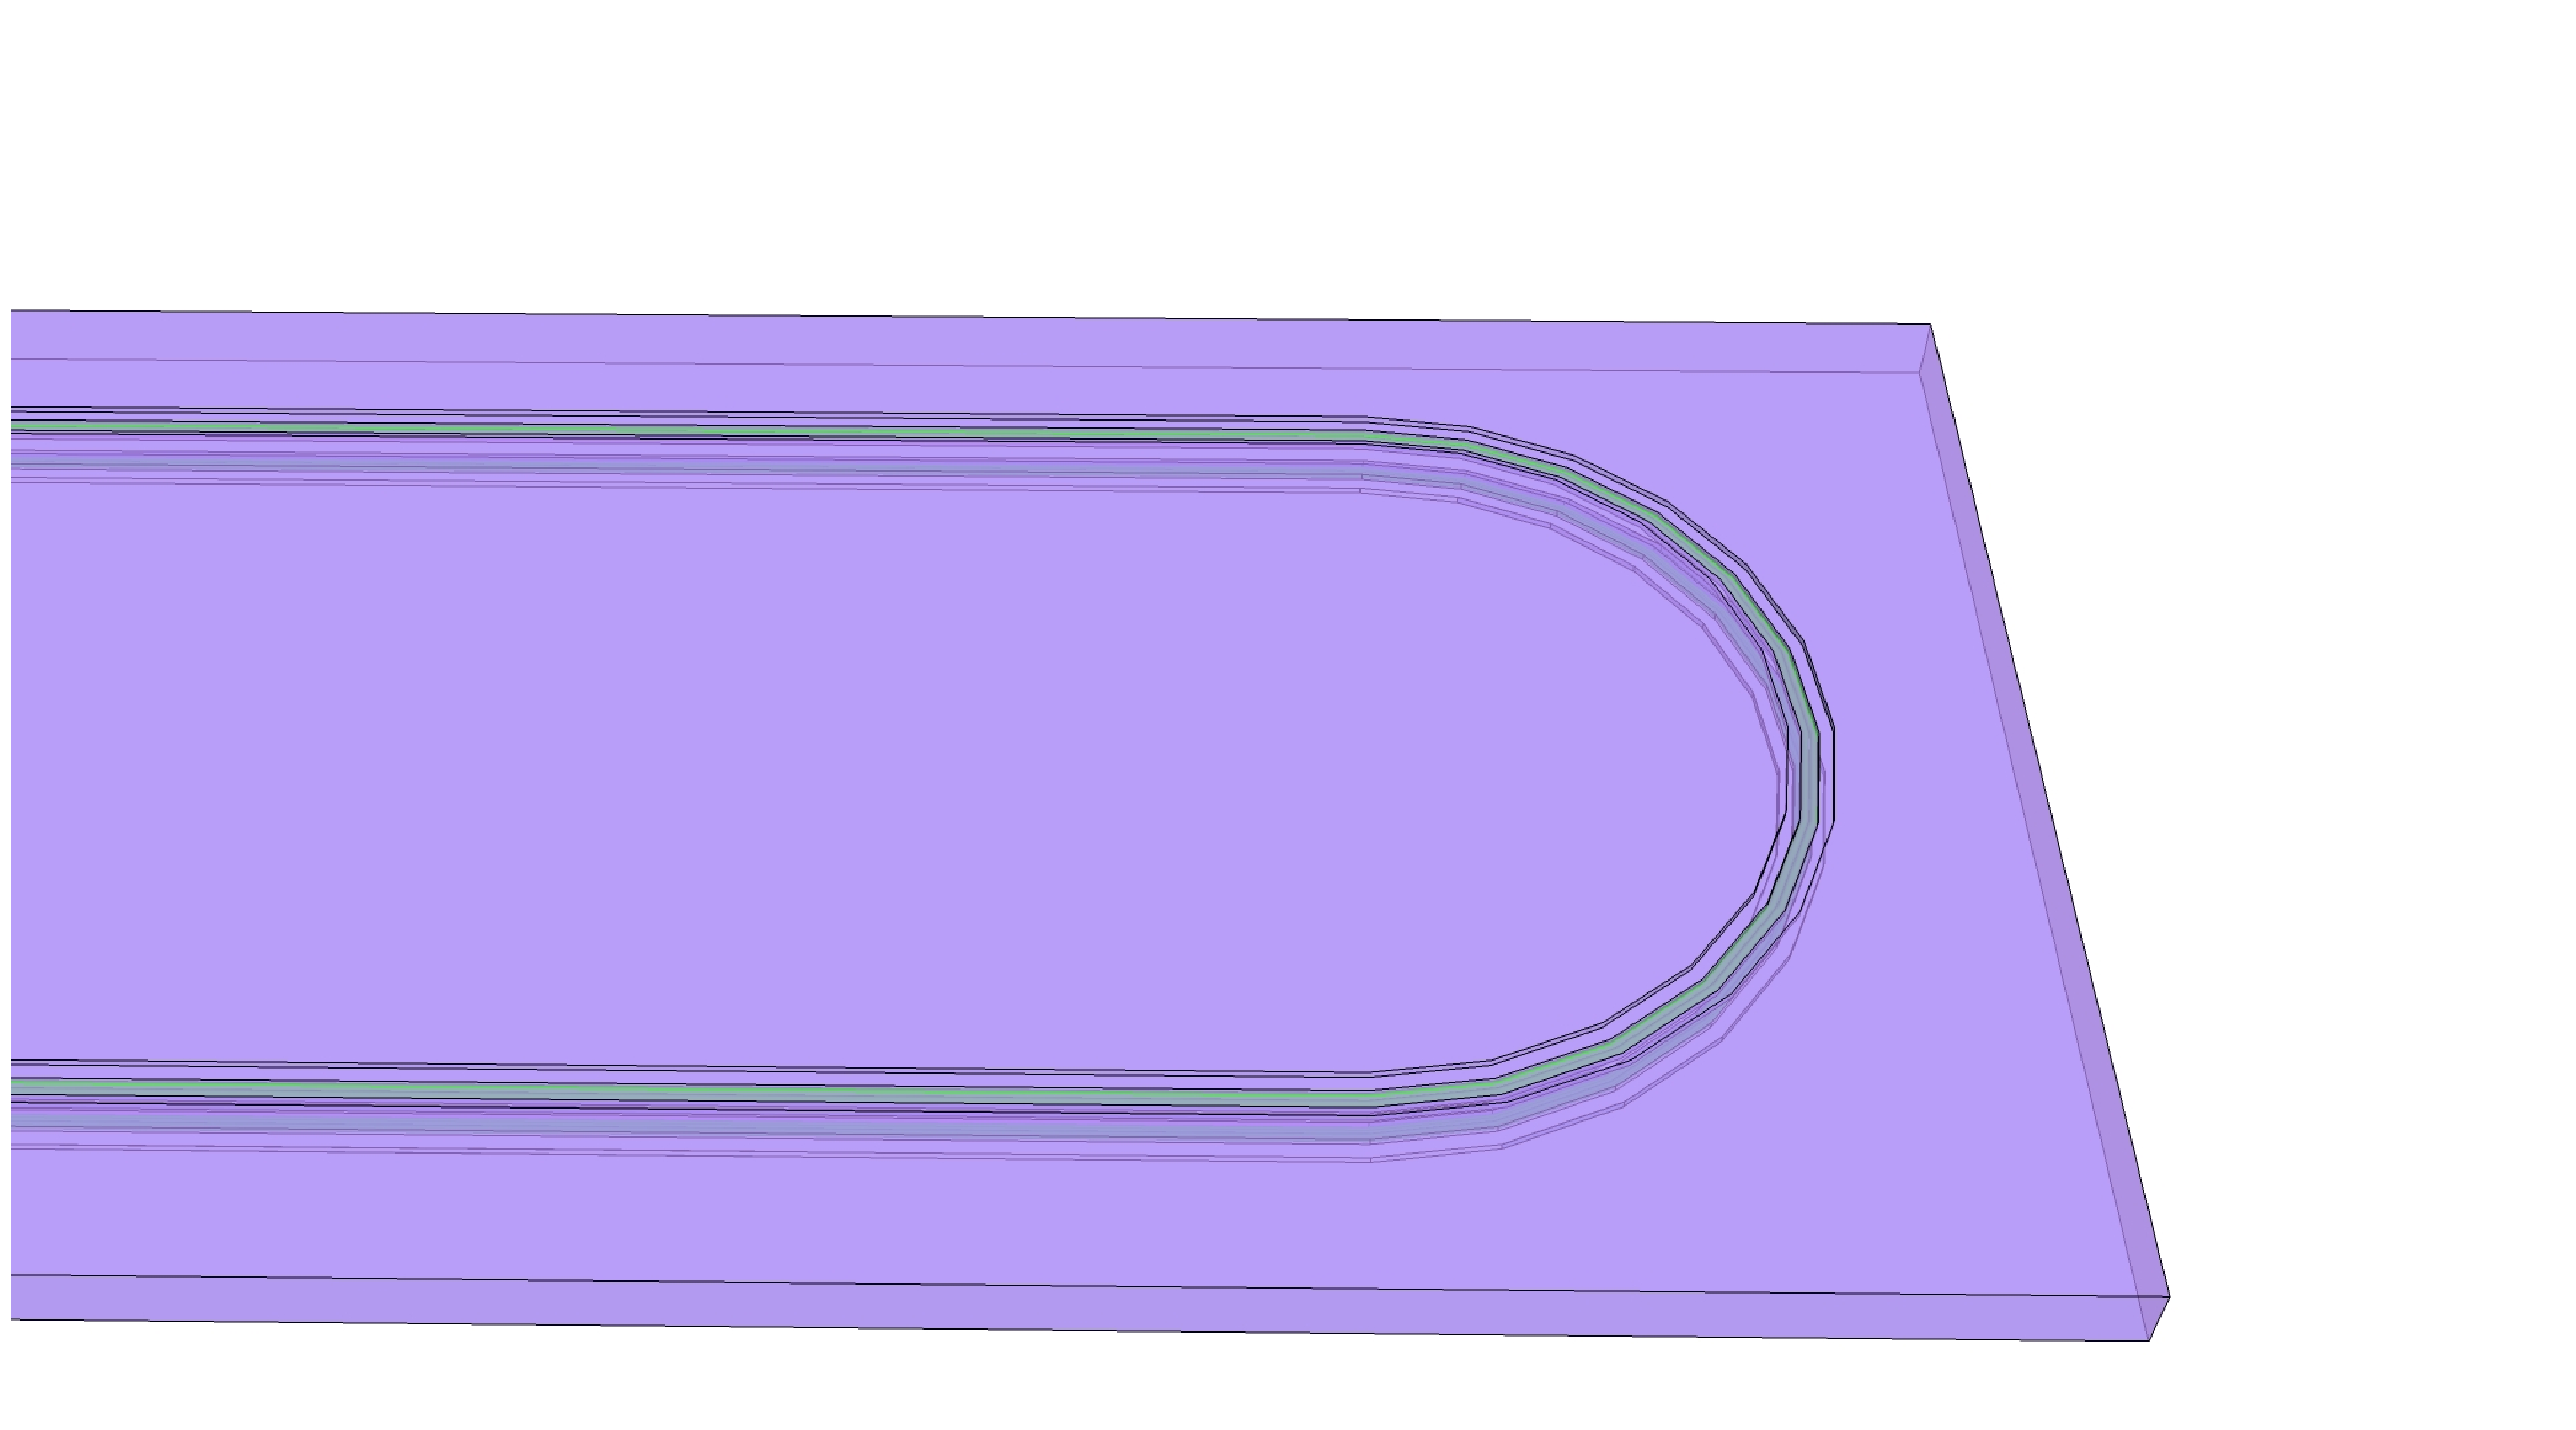
\includegraphics[width=0.5\textwidth]{figures/veto_end.eps}
\caption{The WLS is glued to the scintillator in a ``U'' shape to maximize light recovery.}
\label{fig:paddle}
\end{figure}

An endcap fitted to the scintillator helps protect the WLS and also fixes its location, allowing good alignment to the fibers in the cable.  The endcap also minimizes possible WLS flexing by connecting to machined indents in the scintillator with a press fit.  Because the endcap extends into the scintillator, bending of the fiber perpendicular to its axis is essentially eliminated.  Scintillator material is also machined away from the fiber entrance to the endcap to avoid point pressure.  This ``ramping'' can be shown in {\fig}~\ref{fig:paddleAssembly}.  Once the endcap is slid onto the scintillator, it is glued in place.  This glue is needed because holes the WLS fiber travels through have a small clearance so that threading the endcap does not strip the cladding from the WLS fiber or otherwise damage it, which means that the fibers are slightly loose in their housing.  To optimize light transmission from the WLS fibers to the cable fiber, the surface is polished with a bull-nose, single-crystal diamond.  Gluing the fibers secures them in place so that this polishing does not damage the fiber.  
\begin{figure}[htp]
\centering
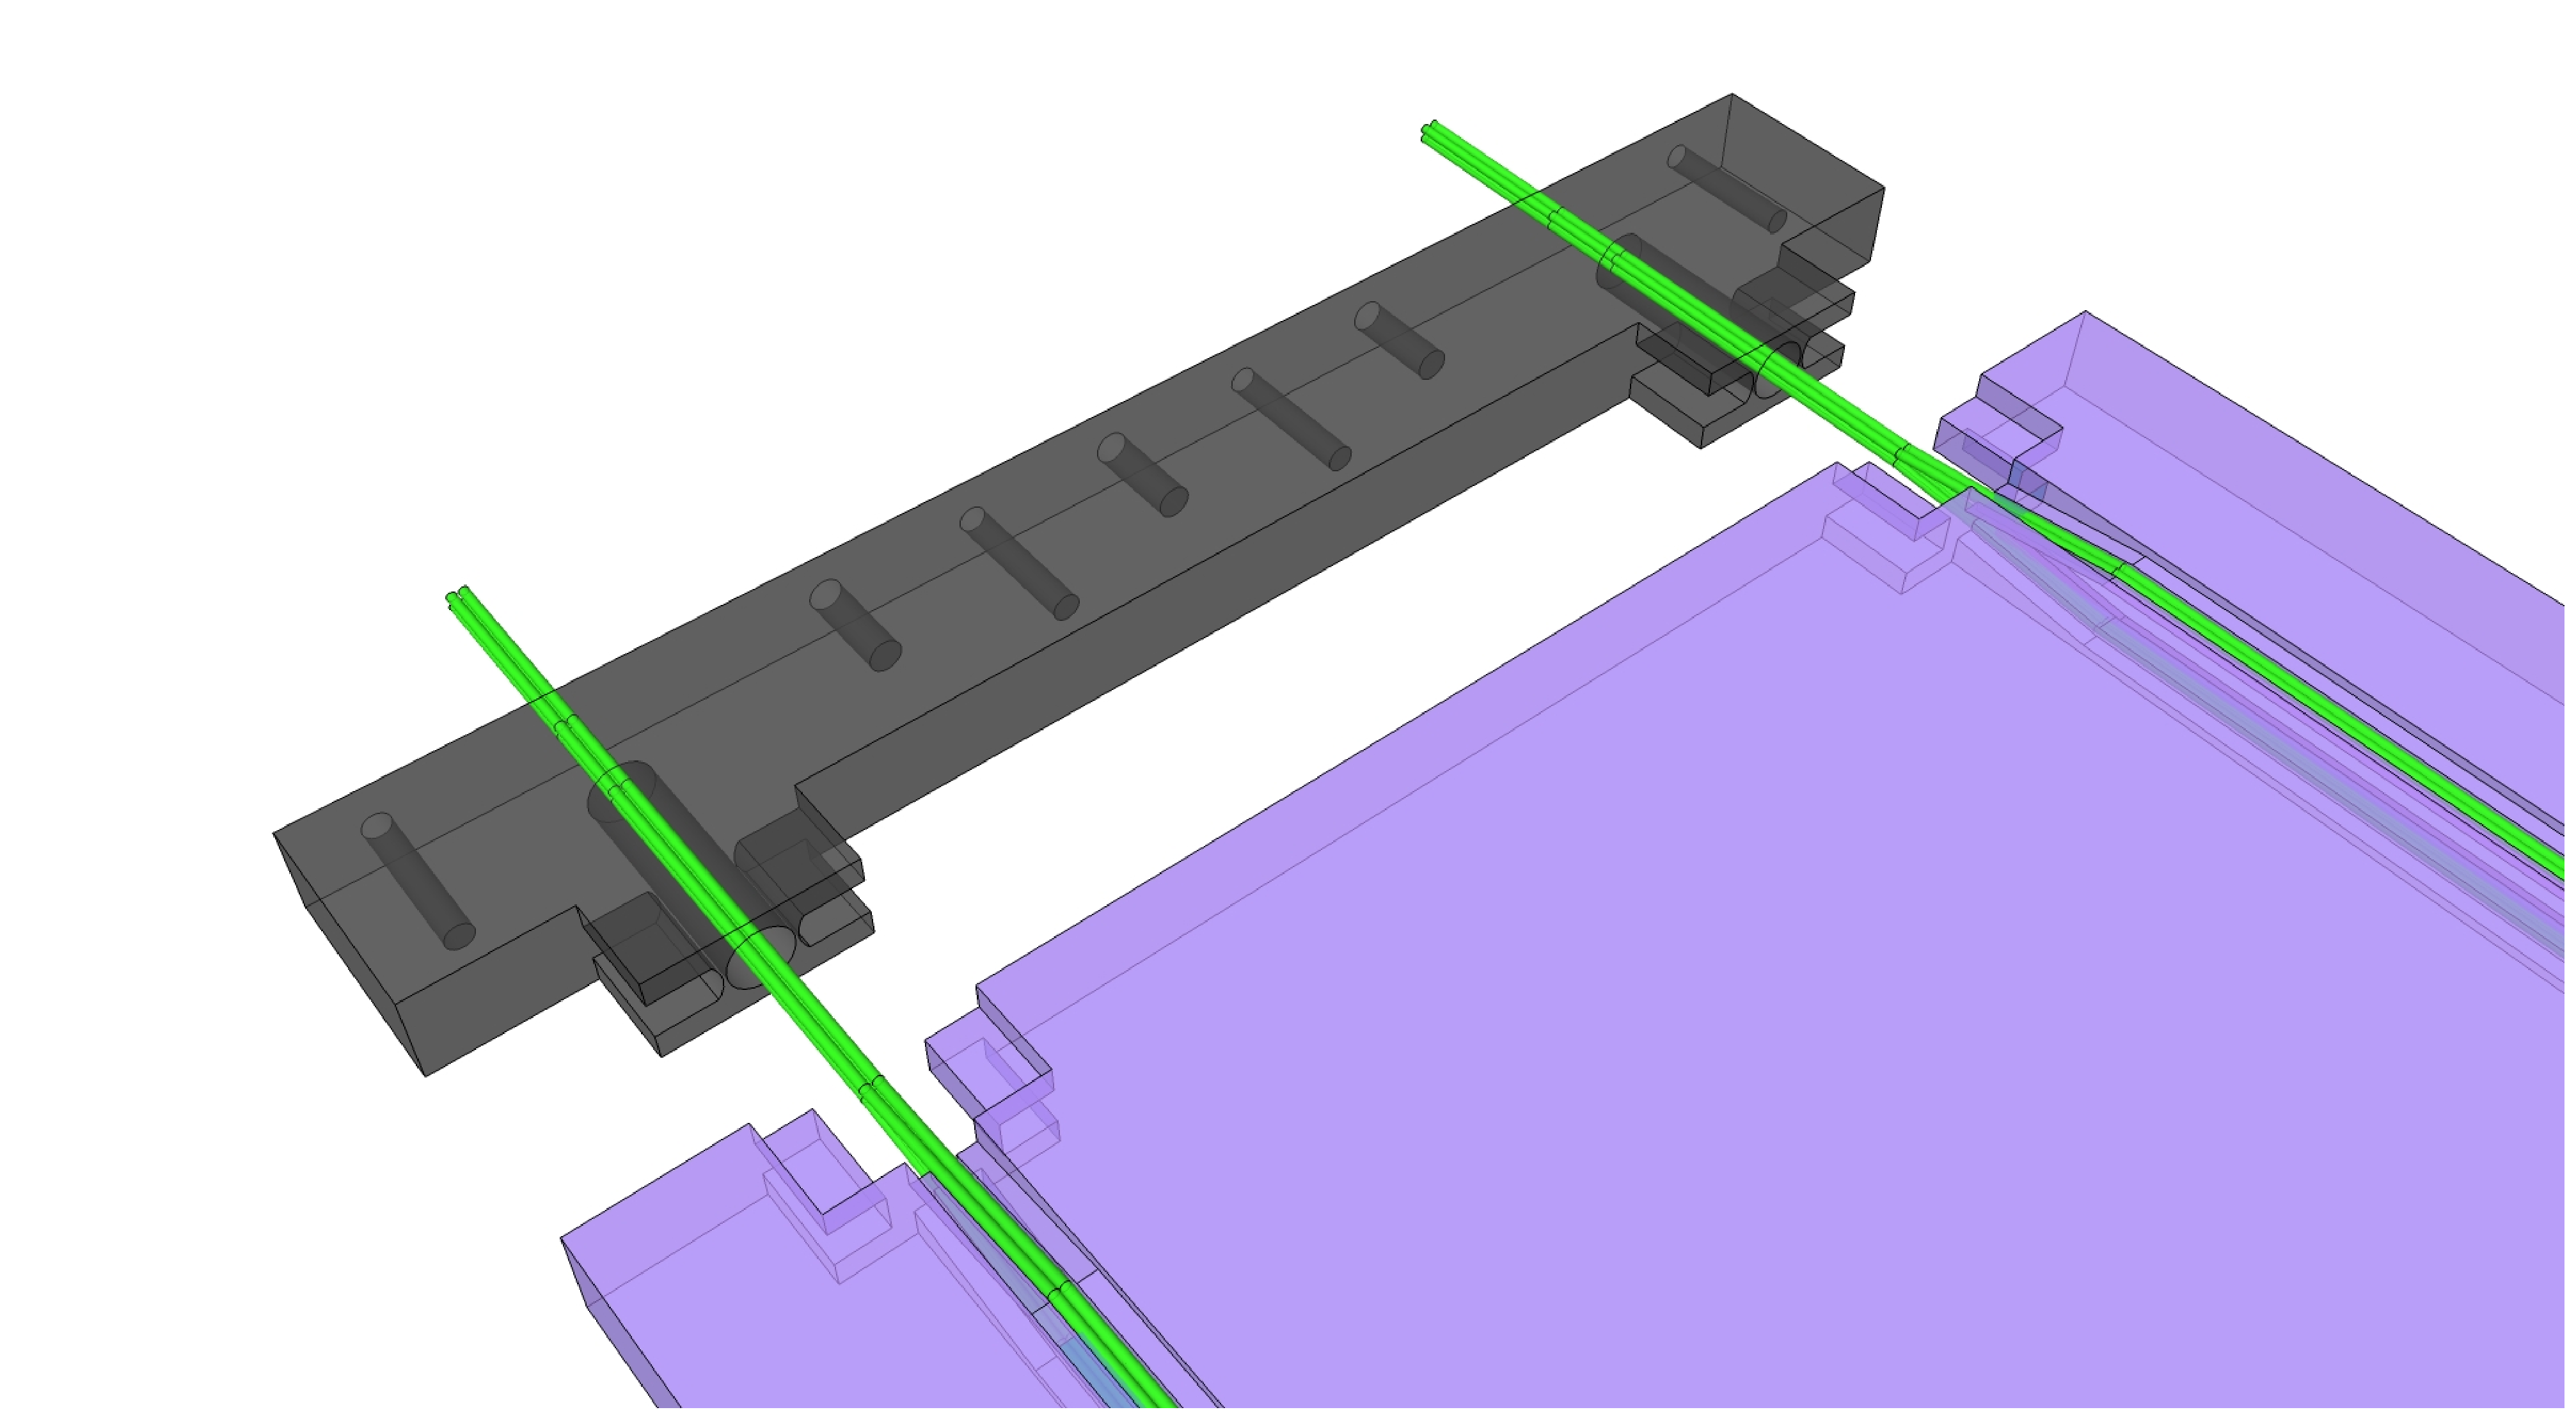
\includegraphics[width=1.0\textwidth]{figures/veto_assembly.eps}
\caption{The endcap is glued to the scintillator after it is slid into place to secure the WLS fibers.}
\label{fig:paddleAssembly}
\end{figure}

The cable consists of two groups of four-clusters of optical fiber, one group for each of the four-clusters of WLS fiber exiting the scintillator.  Optical fiber is preferable to WLS fiber because it is optimized for transmission and is also more durable.  The cable housing must ensure that each transmission fiber completely overlap its WLS fiber and also that the fiber is protected from damage en route to the PMT.  To accomplish this, the cable consists of two types of connectors, one that mates with the endcap attached to the scintillator and another that connects to the PMT, each connected by slightly stiff tubing (durometer = ??) that encases the 2~m long optical fibers.  This tubing helps protect the optical fiber by limiting its bend radius.  At each interface between tubing and connector, the primary concern is that the stresses on the transmission fiber be small enough to avoid damaging the fiber.  A hose barb attached to each connector allows the transmission fiber through and also allows the tubing to firmly connect without putting strain on the fiber.  A cable is shown in {\fig}~\ref{fig:paddleCable}.  Each cable has two groups of optical fiber that connect separately to a cap on the PMT.  Each PMT cap can accept four independent cable connections, allowing two veto paddles to be instrumented by one PMT.  All materials used are black delrin, which is an opaque plastic that is stiff enough to be suitable for machining and also contributes to the light-tightness of the cable.  
\begin{figure}[htp]
\centering
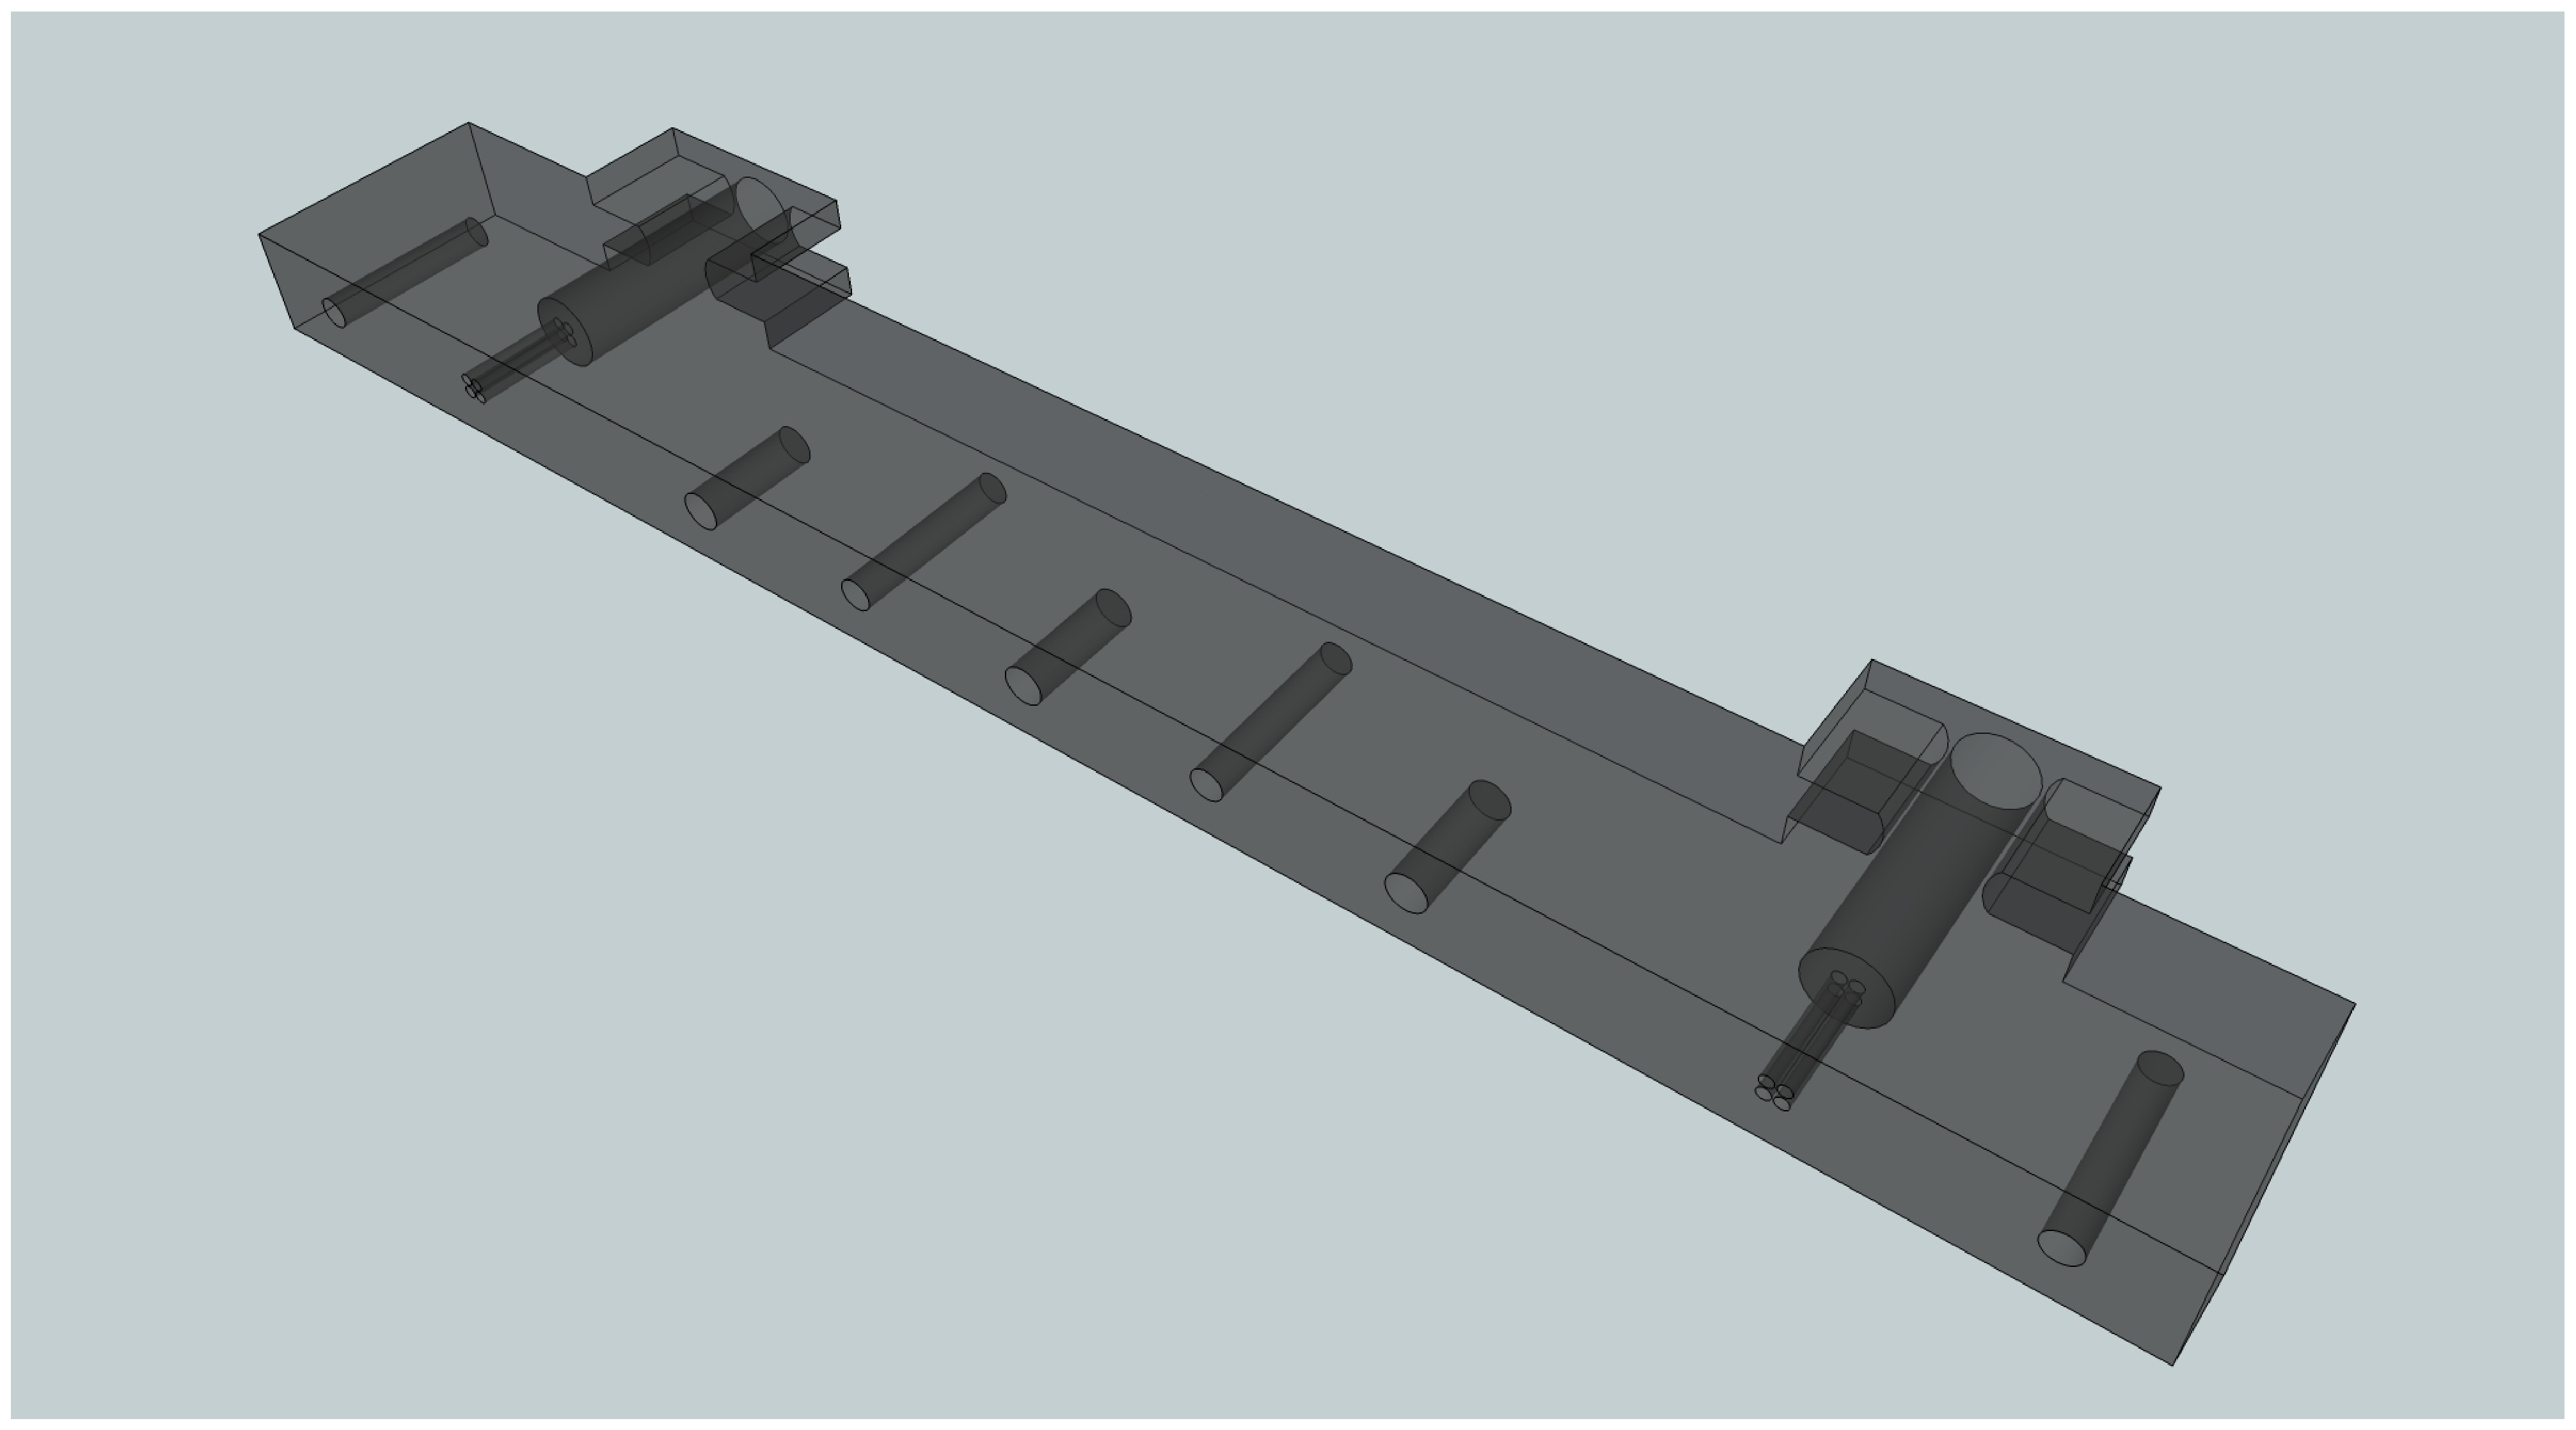
\includegraphics[width=1.0\textwidth]{figures/paddle_connector.eps}
\caption{The cable connector must align with the WLS on the endcap.}
\label{fig:paddleCable}
\end{figure}

The primary design constraint for the portion of the cable that attaches to the endcap is that each transmission fiber completely overlap its WLS fiber.  The diameter of the transmission fiber is 1.2~mm, larger than the 1~mm-diameter WLS fiber, which allows misalignment up to 0.1~mm without greatly impacting light collection.  Tight-fitting dowels help align the region of the cables containing the fiber cluster.  This is particularly important because the connectors are machined from plastic and are not perfectly square - some connectors bow as much as 0.5~mm from normal.  The only regions that must be carefully aligned, however, are the fiber clusters, and the dowels ensure accurate alignment.  Like the WLS fibers in the endcap, the optical fibers must be glued in place so that the mating surface can be diamond-polished without damage.  

The connector that terminates at the PMT is cylindrical to make machining of the PMT cap simple.  In contrast to the endcap connector, the PMT connector has minimal constraints on the position of the optical fibers because the entire 5~cm-diameter PMT face is sensitive to light.  The end of the PMT connector, like the endcap and the endcap connector, is diamond-polished to maximize optical coupling, and so the fiber is glued into place to protect it from damage during polishing.    Also like the endcap connector, strain relief is provided to the optical cable by attaching the protective tubing to the connector with hose barb, eliminating extreme bending of the optical cable.    
The cap fitted to the face of the PMT has four holes drilled with a diameter that provides a press-fit with the PMT connectors from the cable.  The cap fits snugly onto the PMT so that the optical cables in the PMT connectors are held securely to the surface of the PMT.  The diamond polishing results in a very uniform surface and it was found that applying optical grease to the connection did not result in noticeable improvement.  The coupling to the PMT was therefore left as an air coupling.  One way to improve light collection by the PMT was to connect the optical fibers to PMT closer to the center of the PMT face.  This was done by machining PMT caps with the holes for the connectors drilled as closely as allowed by the plastic, $\sim$2~mm.


\section{Paddle Performance}
\label{sec:singleVeto}

%\subsection{tests on intrinsic efficiency}
\begin{comment}
Show signal from detector
Talk about first tests?  Can talk about sensitivity to geometric alignment of trigger paddles ...
Maybe mention this and then be like, ``this is why we decided to look at the efficiency this other way that was less sensitive''
except you weren't able to do further tests so you'll just have to say the limits you got
\begin{figure}[htp]
\centering
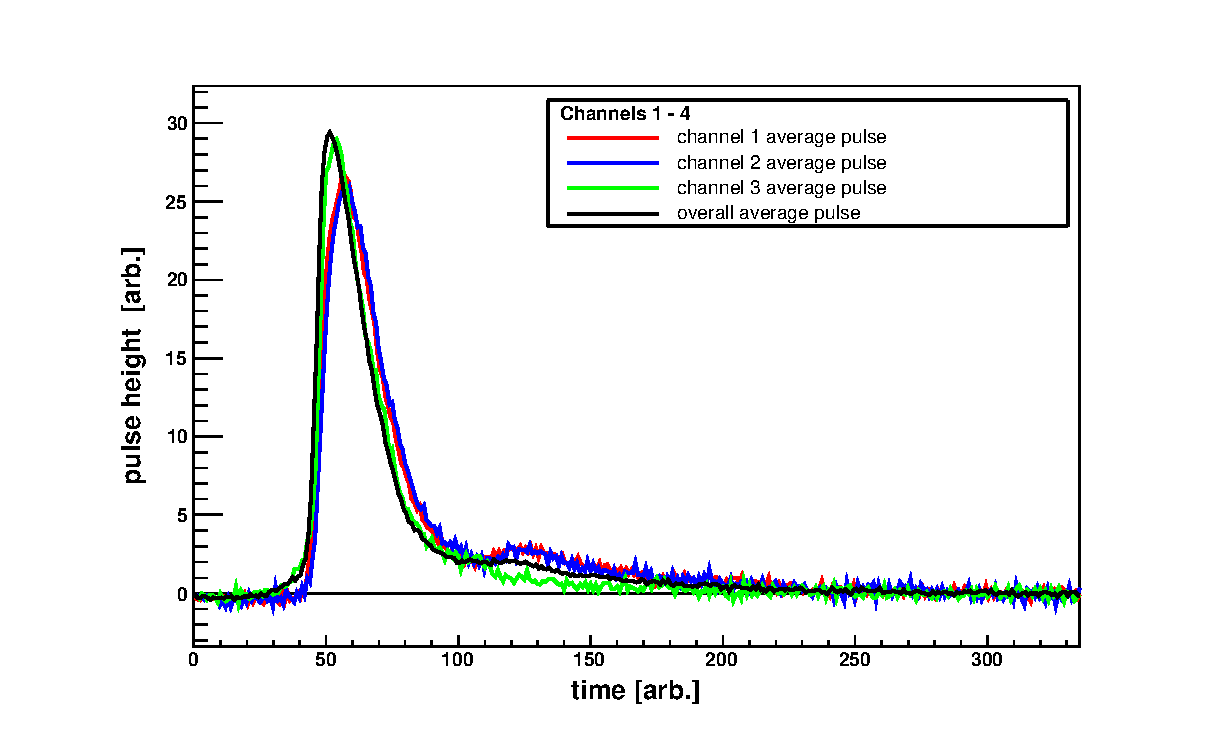
\includegraphics[width=0.5\textwidth]{figures/PulseChan_1_4.eps}
\caption{Pulses from muons in the veto paddles.}
\label{fig:vetoSignal}
\end{figure}
\end{comment}
The intrinsic efficiency of the paddles can be tested by requiring a coincidence with several paddles.  The several-detector coincidence identifies signals as muons.  If the coincidence paddles are arranged so that the path of any muon intersecting all the veto paddles must also intersect the volume of the veto paddle, the intrinsic efficiency of the veto paddle can be measured separate from its geometric coverage.

In practice, arranging the available scintillators to confine muon paths through the test volume was difficult because the available scintillator was instrumented with bulky lightguides and could not be laid directly on the test volume.  A simple cosmic-ray simulation program helped determine an arrangement that guaranteed a geometrical efficiency of at least 99\%.  This arrangement is shown in {\fig}~\ref{fig:efficiencyTest}.  Note that the coincidence paddles are slightly wider than the veto paddle, which requires the coincidence paddles to be aligned to each edge of the veto paddle.  
\begin{figure}[htp]
\centering
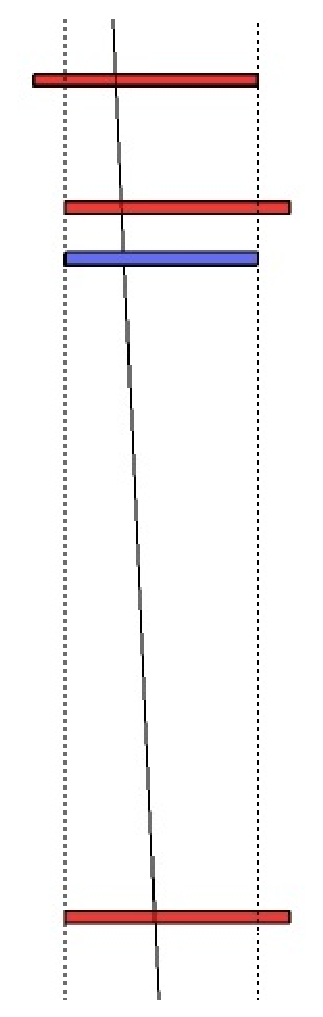
\includegraphics[height=0.4\textheight]{figures/veto_test_layout.eps}
\caption{This arrangement of coincidence material ensures that muons triggering all coincidence detectors must also travel through the veto paddle.  The coincidence material is drawn in red while the veto paddle is in blue.}
\label{fig:efficiencyTest}
\end{figure}

The efficiency was measured by counting how often the veto paddle had a detectable signal when all the coincidence paddles registered a coincidence.  Assuming that the muon is thereby constrained to travel through the veto paddle volume, the ratio gives the intrinsic efficiency.  The DAQ Event signal was a logic pulse resulting from the coincidence of the coincidence paddles.  This logic pulse also acted as a start for a time-to-amplitude converter (TAC).  The TAC stop signal was a delayed, discriminated veto paddle signal.  The outgoing TAC signal was then sent to an analog to digital converter (ADC), which integrates the signal.  Signals from the veto paddle coincident with the other scintillators appear in the timing spectrum as a peak at the time of the delay.  The integral of this timing peak divided by the number of event triggers gives the efficiency.
% figure: the considerably complicated spectrum
\begin{figure}[htp]
\centering
\subfloat[][]{
   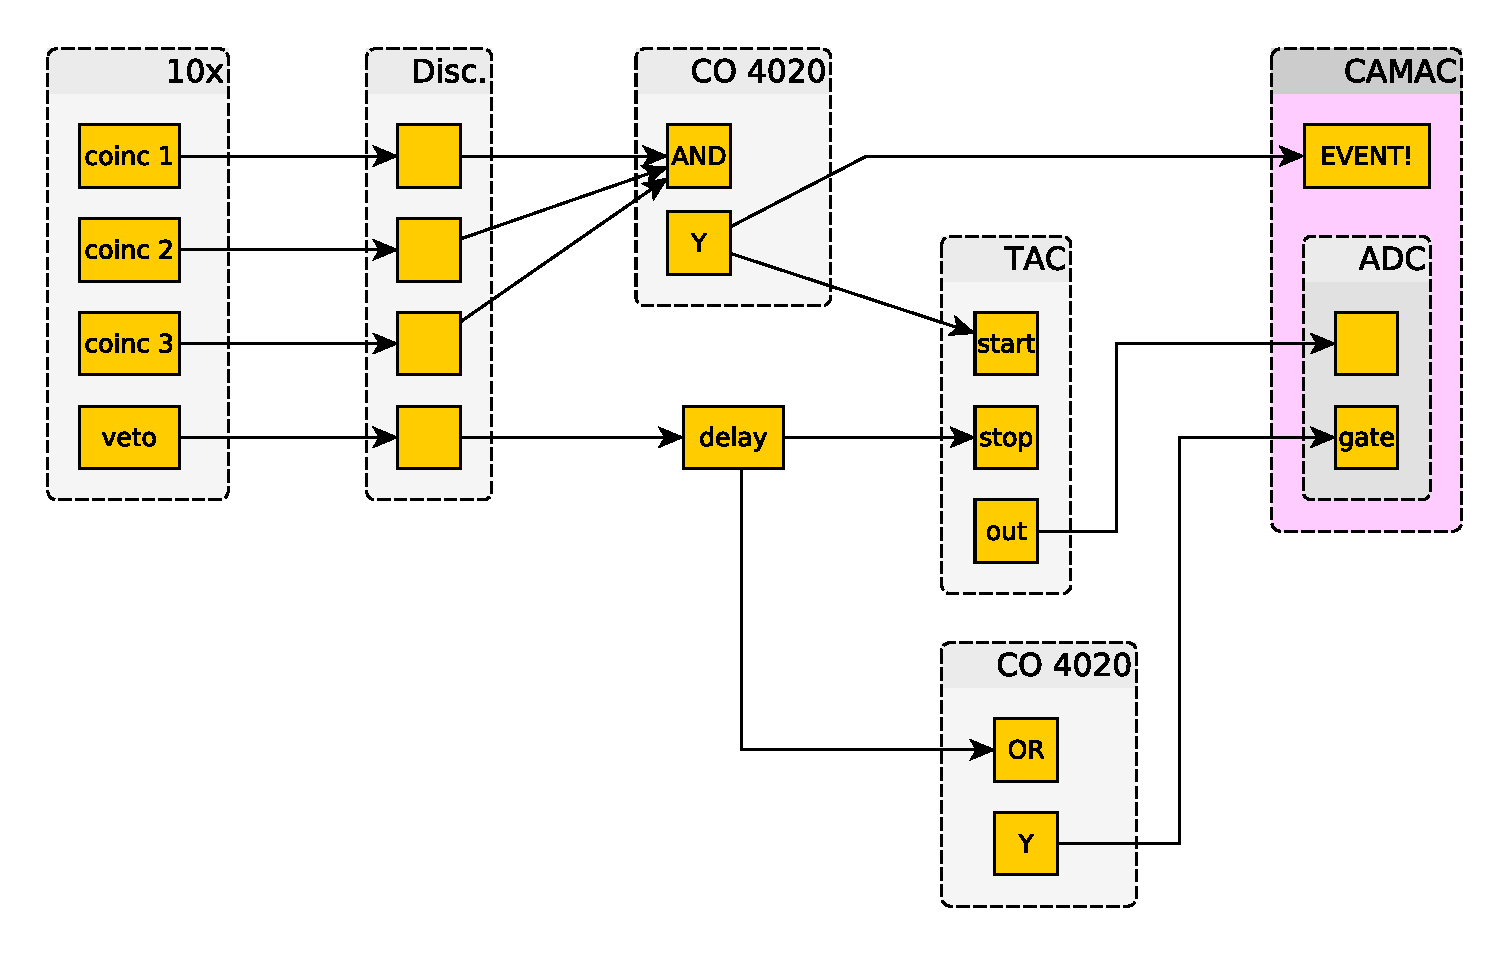
\includegraphics[width=0.45\textwidth]{figures/electronics_vetoTest.eps}	
}
\subfloat[][]{
	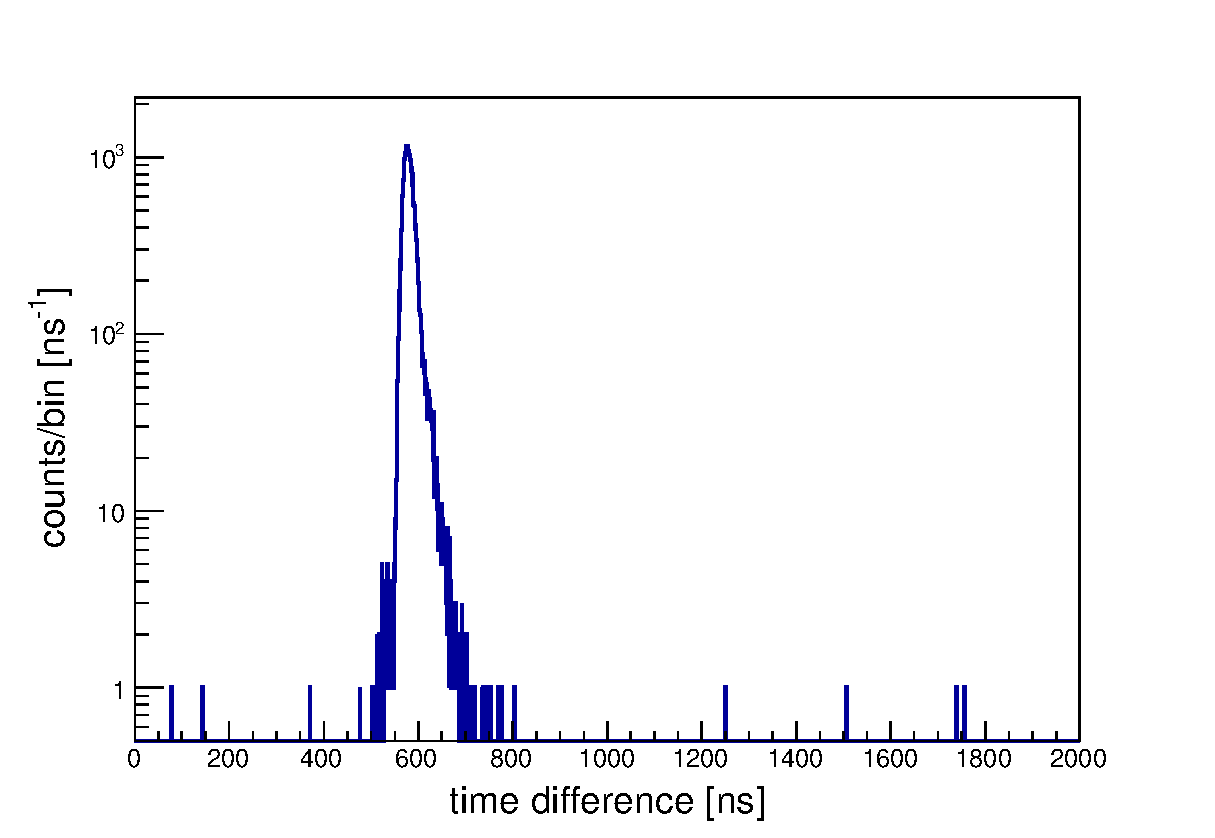
\includegraphics[width=0.45\textwidth]{figures/efficiencyTest_timingSpectrum.eps}
}
\caption{The location of the timing peak is set by the delay introduced to the discriminated veto paddle signal.  Integrating the timing peak gives the number of muons that generated an observable signal in the veto paddle.}
\label{fig:vetoTestElectronics}
\end{figure}

Testing the efficiency of the veto paddle with this setup was not ideal because the geometrical efficiency was very sensitive to the placement of the coincidence detectors.  The measured efficiency of the same bar could change from 98\% to 75\% when the middle coincidence detector was shifted away from the edge of the veto paddle by as little as a few centimeters.  However, this setup was useful in testing the effect of the cable polishing, cable out-of-true-ness, and the condition of the plastic scintillator.  In general, all efficiency measurements fell between 94\% and 98\%.  Even the veto paddles made of plastic with deep internal cracks were as efficient as the veto paddles made from the plastic in excellent condition.  No statistically significant differences were seen between cables made with badly bowed connectors and nearly true connectors.  Polishing the cables with the bull-nose single-crystal diamond rather than a commonly-available multi-crystal diamond bit increases detection efficiency by $\sim2$\%, although it should be noted that the change may have been due to correlated noise in the system rather than to improved light transmission.  The discriminator threshold, set to its lowest value, gave an efficiency of 98\% compared to 94\% when set to its highest value.

Testing the position dependence of the efficiency using the setup described above was not practical due to its sensitivity on positioning.  Instead, the response of the veto paddles to a loosely collimated $\gamma$ source was tested.  A $^{60}$Co source was inserted into a 3 cm thick lead ring and raised 2~cm within the ring by a small piece of plastic.  This collimated source was then placed at three positions along the veto paddle, near the endcap, at the middle of the paddle, and near the end of the paddle.  Several measurements were taken at different horizontal positions in the center of the veto paddle. The detected rate of $\gamma$ radiation showed a deviation of less than 10\% over the veto paddle.  While this is not a measurement of the position dependence of the muon efficiency, it does limit the efficiency change over the paddle since muons typically deposit at least twice the energy of the $\gamma$ radiation from the $^{60}$Co source.  See {\fig}~\ref{fig:positionDependence} for the variation of the efficiencies.
\begin{figure}[htp]
\centering
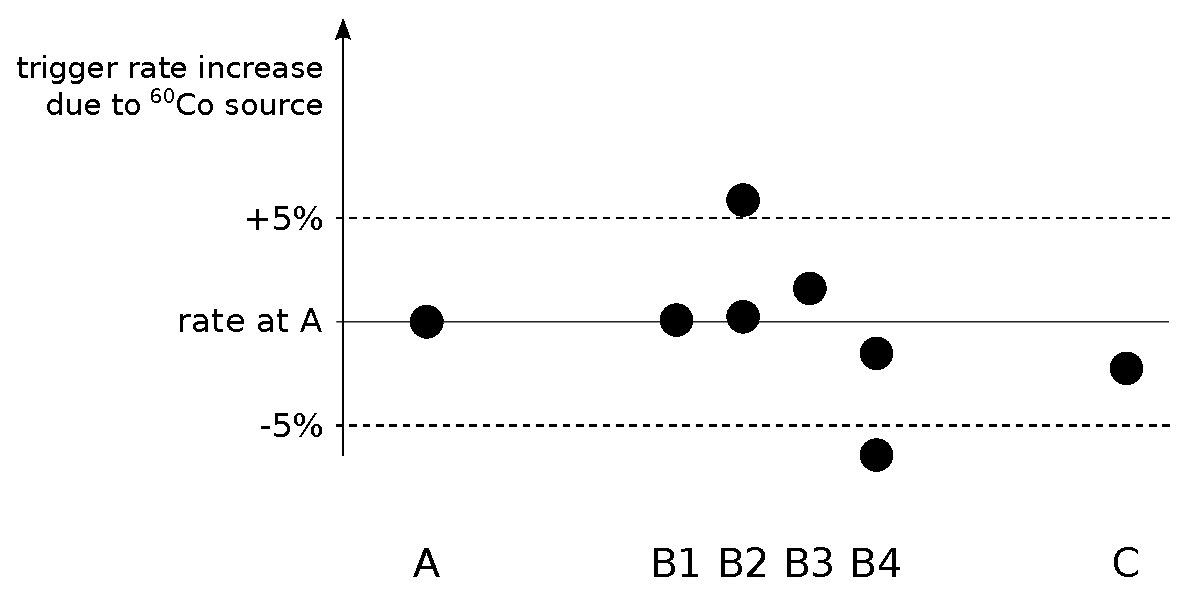
\includegraphics[width=1.0\textwidth]{figures/efficiency_positionDependence.eps}
\caption{The dependence of the number of detected events on the position of a loosely-collimated $^{60}$Co source.  Positions A and C are closest and furthest from the cable connection, respectively.  Position B is the center of the veto paddle.  Data was taken in the center across the bar to test for horizontal position dependence.  The position B1 is at the horizontal center and B4 is at the edge of the veto paddle.  Several measurements were taken at B2 and B3, the points nearest the WLS fiber channel.  The spread is approximately 10\%.}
\label{fig:positionDependence}
\end{figure}


\subsection{On-Detector Efficiency}
\begin{comment}
Initial efficiency - would be nice to show this data
Describe different cosmics that hit the neutron bar but miss the veto - argh!
Discuss changes made to mounting to improve coverage - show new data (cosmics)
\end{comment}
Sixteen veto paddles were initially mounted $\sim$2~cm in front of the neutron detector bars to avoid removing (and potentially damaging) the heavy neutron detector bars.  Running a test with \MgReaction showed good muon rejection in the two innermost bars of each four-bar unit and worse rejection in the outer two bars by about 20\%.  The outer bars act as additional veto material for the inner bars, while the outer bars have no such additional information to aid in muon identification.  It should be noted that adjacent veto paddles were instrumented by a single PMT, making it impossible to distinguish veto signals from distinct veto paddles.  
\begin{figure}[htp]
%\centering
%\includegraphics[width=1.0\textwidth]{figures/initialBackground.eps}
\vspace{3in}
\caption{Room background after rejection with the initial placement of the veto paddles.  Note that the high-background bars are those on the ends of each group of four.}
\label{fig:initialBackground}
\end{figure}

A simulation of the muon background indicated that the geometrical efficiency was very sensitive to the distance between the veto paddle and neutron detector bar as well as the distance between the bars of the neutron detector.   The bars in the neutron detector were moved as close as the mounting screws would allow, within 1~cm.  Instead of attaching the veto paddles on top of the retaining bars on the neutron detector, they were taped to the bars and both bar and veto paddle were supported together by the same retaining bar.  The separation between the bars of the neutron detector and their veto paddle is $\sim$0.5~cm due to stiff foam placed between the two to protect the WLS channels in the veto paddles.  Material was also added to the sides of the outermost neutron detectors.  The final setup is shown in {\fig}~\ref{fig:vetoSetup}.  These changes improved both the average and uniformity of the background rejection, as can be seen in {\fig}~\ref{fig:finalBackground}.
\begin{figure}[htp]
\centering
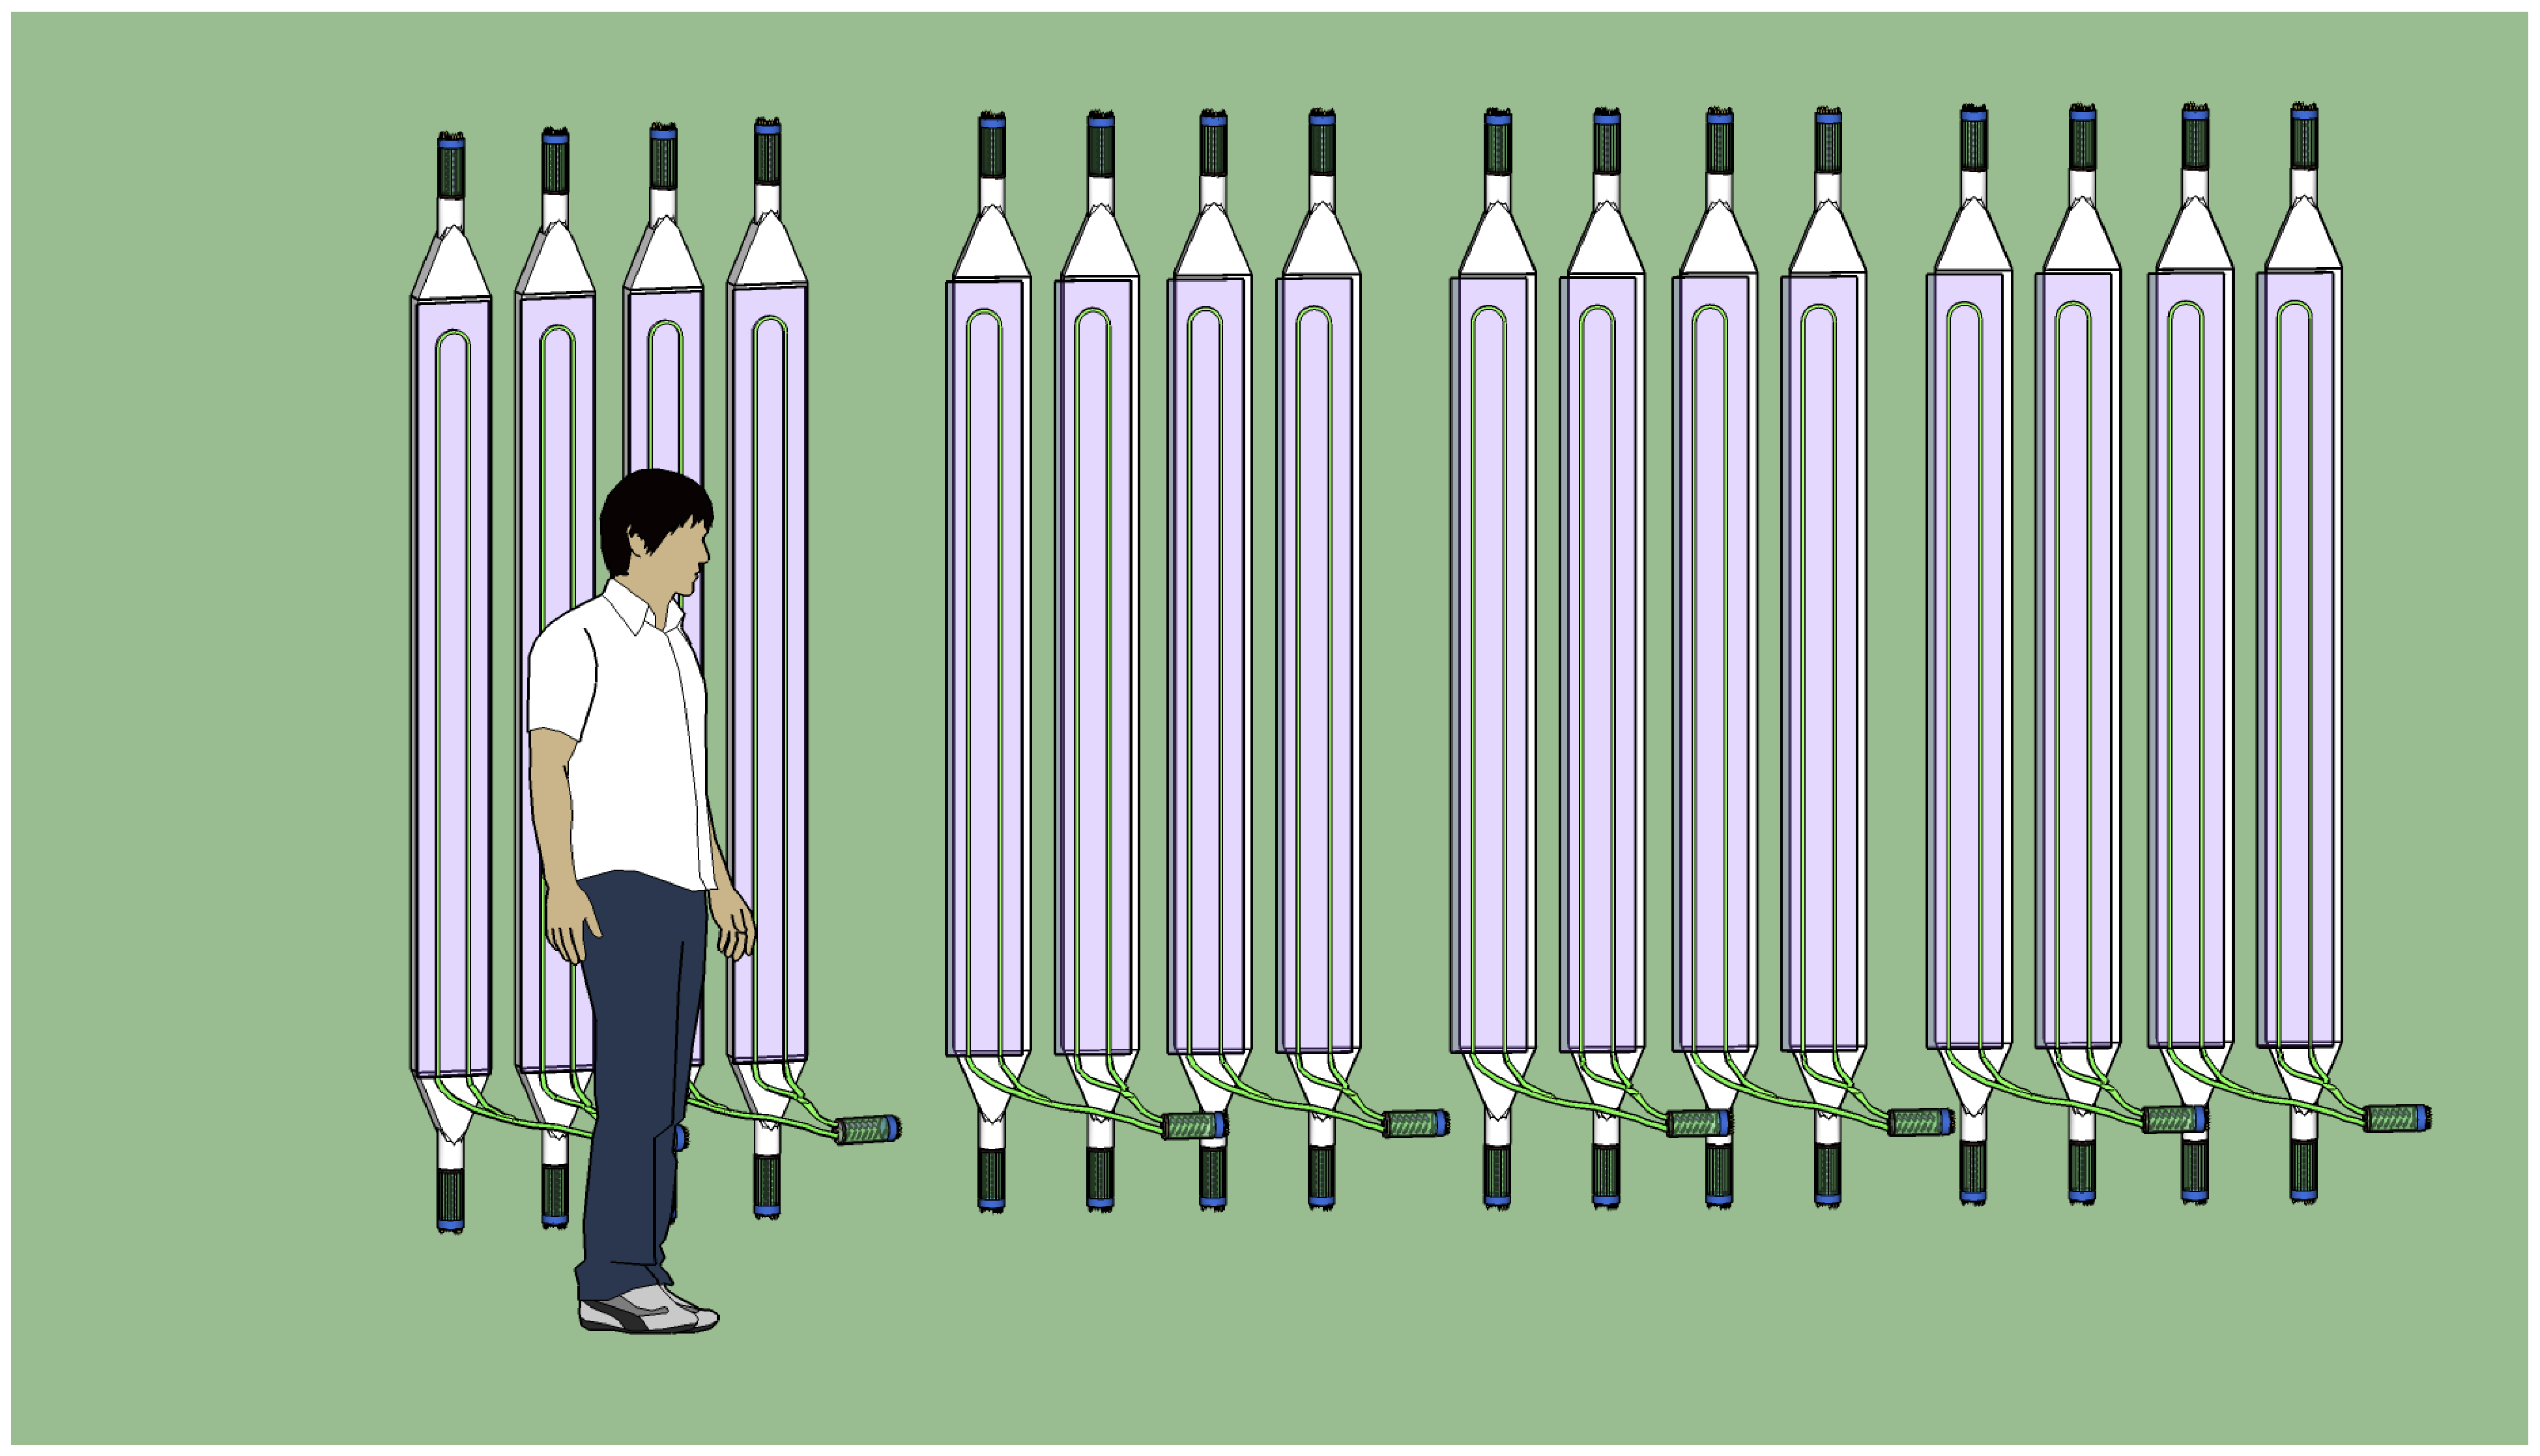
\includegraphics[width=1.0\textwidth]{figures/neutwall_Oct18.eps}
\caption{The final arrangement of the veto paddles on the neutron detector.  The distance between the veto paddles and the bars of the neutron detector have been minimized.  Note also the addition of veto material on the sides of the neutron detector sub-units.}
\label{fig:vetoSetup}
\end{figure}

\begin{figure}[htp]
%\centering
%\includegraphics[width=1.0\textwidth]{figures/finalBackground.eps}
\vspace{3in}
\caption{Room background after rejection by the veto.  Note that the average and the spread are both reduced from that of the initial setup.}
\label{fig:finalBackground}
\end{figure}

\section{Electronics}
\begin{comment}
Originally wanted to use timing information but there weren't enough channels
Bit Register - give example
discuss random rate and estimate how often you'll fire during a real event and also how often one bar will fire with something real, vetoing a real event
LeCroy 4532 - MALU - majority logic unit ``The status of up to 32 inputs can be monitored and recorded by issuing a strobe.  Since the inputs are edge-triggered, the strobe may be a gate of arbitrary duration.  Then any inputs which are on during any portion of the gate are recorded and stored in a pattern register.'' (from the manual).
\end{comment}
As mentioned above in {\sect}~\ref{sec:singleVeto}, tests on single veto paddles were done using a timing spectrum.  Recording complete time information for the full veto was not practical, and bit registers were used instead.  A bit register has several inputs, each corresponding to a bit in an integer, and a gate.  When the gate is open, the bit register records the pattern at its inputs.  Each input is connected to a discriminator which fires when the signal from the given veto bar exceeds a threshold.  The result is a unique representation of which bars fired during the time specified by the gate.  If the gate used is the Event signal from the neutron detector, the bit register will record which veto paddles fired during an event of interest.  Two 16-channel LeCroy 4532 bit registers were used to instrument all the veto paddles.  The gate signal was a 200~ns-wide logic signal generated from the event trigger.

Recording the integer generated by the bit register instead of the time of the signal relative to the beam bunch results in a loss of information.  The maximum time difference between an event in the neutron detector and an event in the veto that will still be recorded in the bit pattern is the width of the gate signal, 200~ns.  This compares unfavorably to the timing spectrum, where even with a leading edge discriminator, the timing peak has a width of less than 5~ns.  The concern is that this loss of precision in timing information will lead to unacceptable vetoing of real events.  

Several sources contribute to non-beam-related background radiation, resulting in a beam-off rate in a neutron detector bar of $\sim$1000~Hz.  While some of these events are due to muons, they have a flux of $\sim$10~Hz/m$^2$ and are therefore a small part of the beam-off noise rate.  The beam-off rate, then, serves as a suitable rate with which to calculate an upper bound for the rejection of beam-related events.  The probability that a noise event will occur within the window allowed by the bit register and veto a beam-related event is
\begin{equation}
\text{R}_{\text{noise}}\times\tau_{\text{bit reg.}} = 10^3\text{ Hz}\times200\times10^{-9}\text{ ns} = 2\times10^{-4},
\end{equation}
where $\text{R}_{\text{noise}}$ is the noise rate and $\tau_{\text{bit reg.}}$ is the time window of the bit register.  The bars of the neutron detector experiencing the highest veto noise rate are vetoed by four veto paddles.  Two of these are the veto paddles mounted directly in front of it and the adjacent neutron detector bar, and the other two are the bars on its sides.  The two front veto paddles have a combined noise rate of 1000~Hz, while the two side veto paddles could each have a rate of 1000~Hz, giving a maximum noise rate of 3000~Hz.   The bit register window was set at 200~ns, so that the maximum probability of vetoing a real, beam-induced event is $6\times10^{-4}$, or approximately one false veto per 1500 events.  This fraction of vetoed events is less than 1\% and will not have any statistical significance, even with the timing resolution lost by moving to a bit register.  A schematic of the veto electronics is shown in {\fig}~\ref{fig:vetoElectronics}.  Note that no changes to the DAQ other than the addition of the bit register are required.
\begin{figure}[htp]
\centering
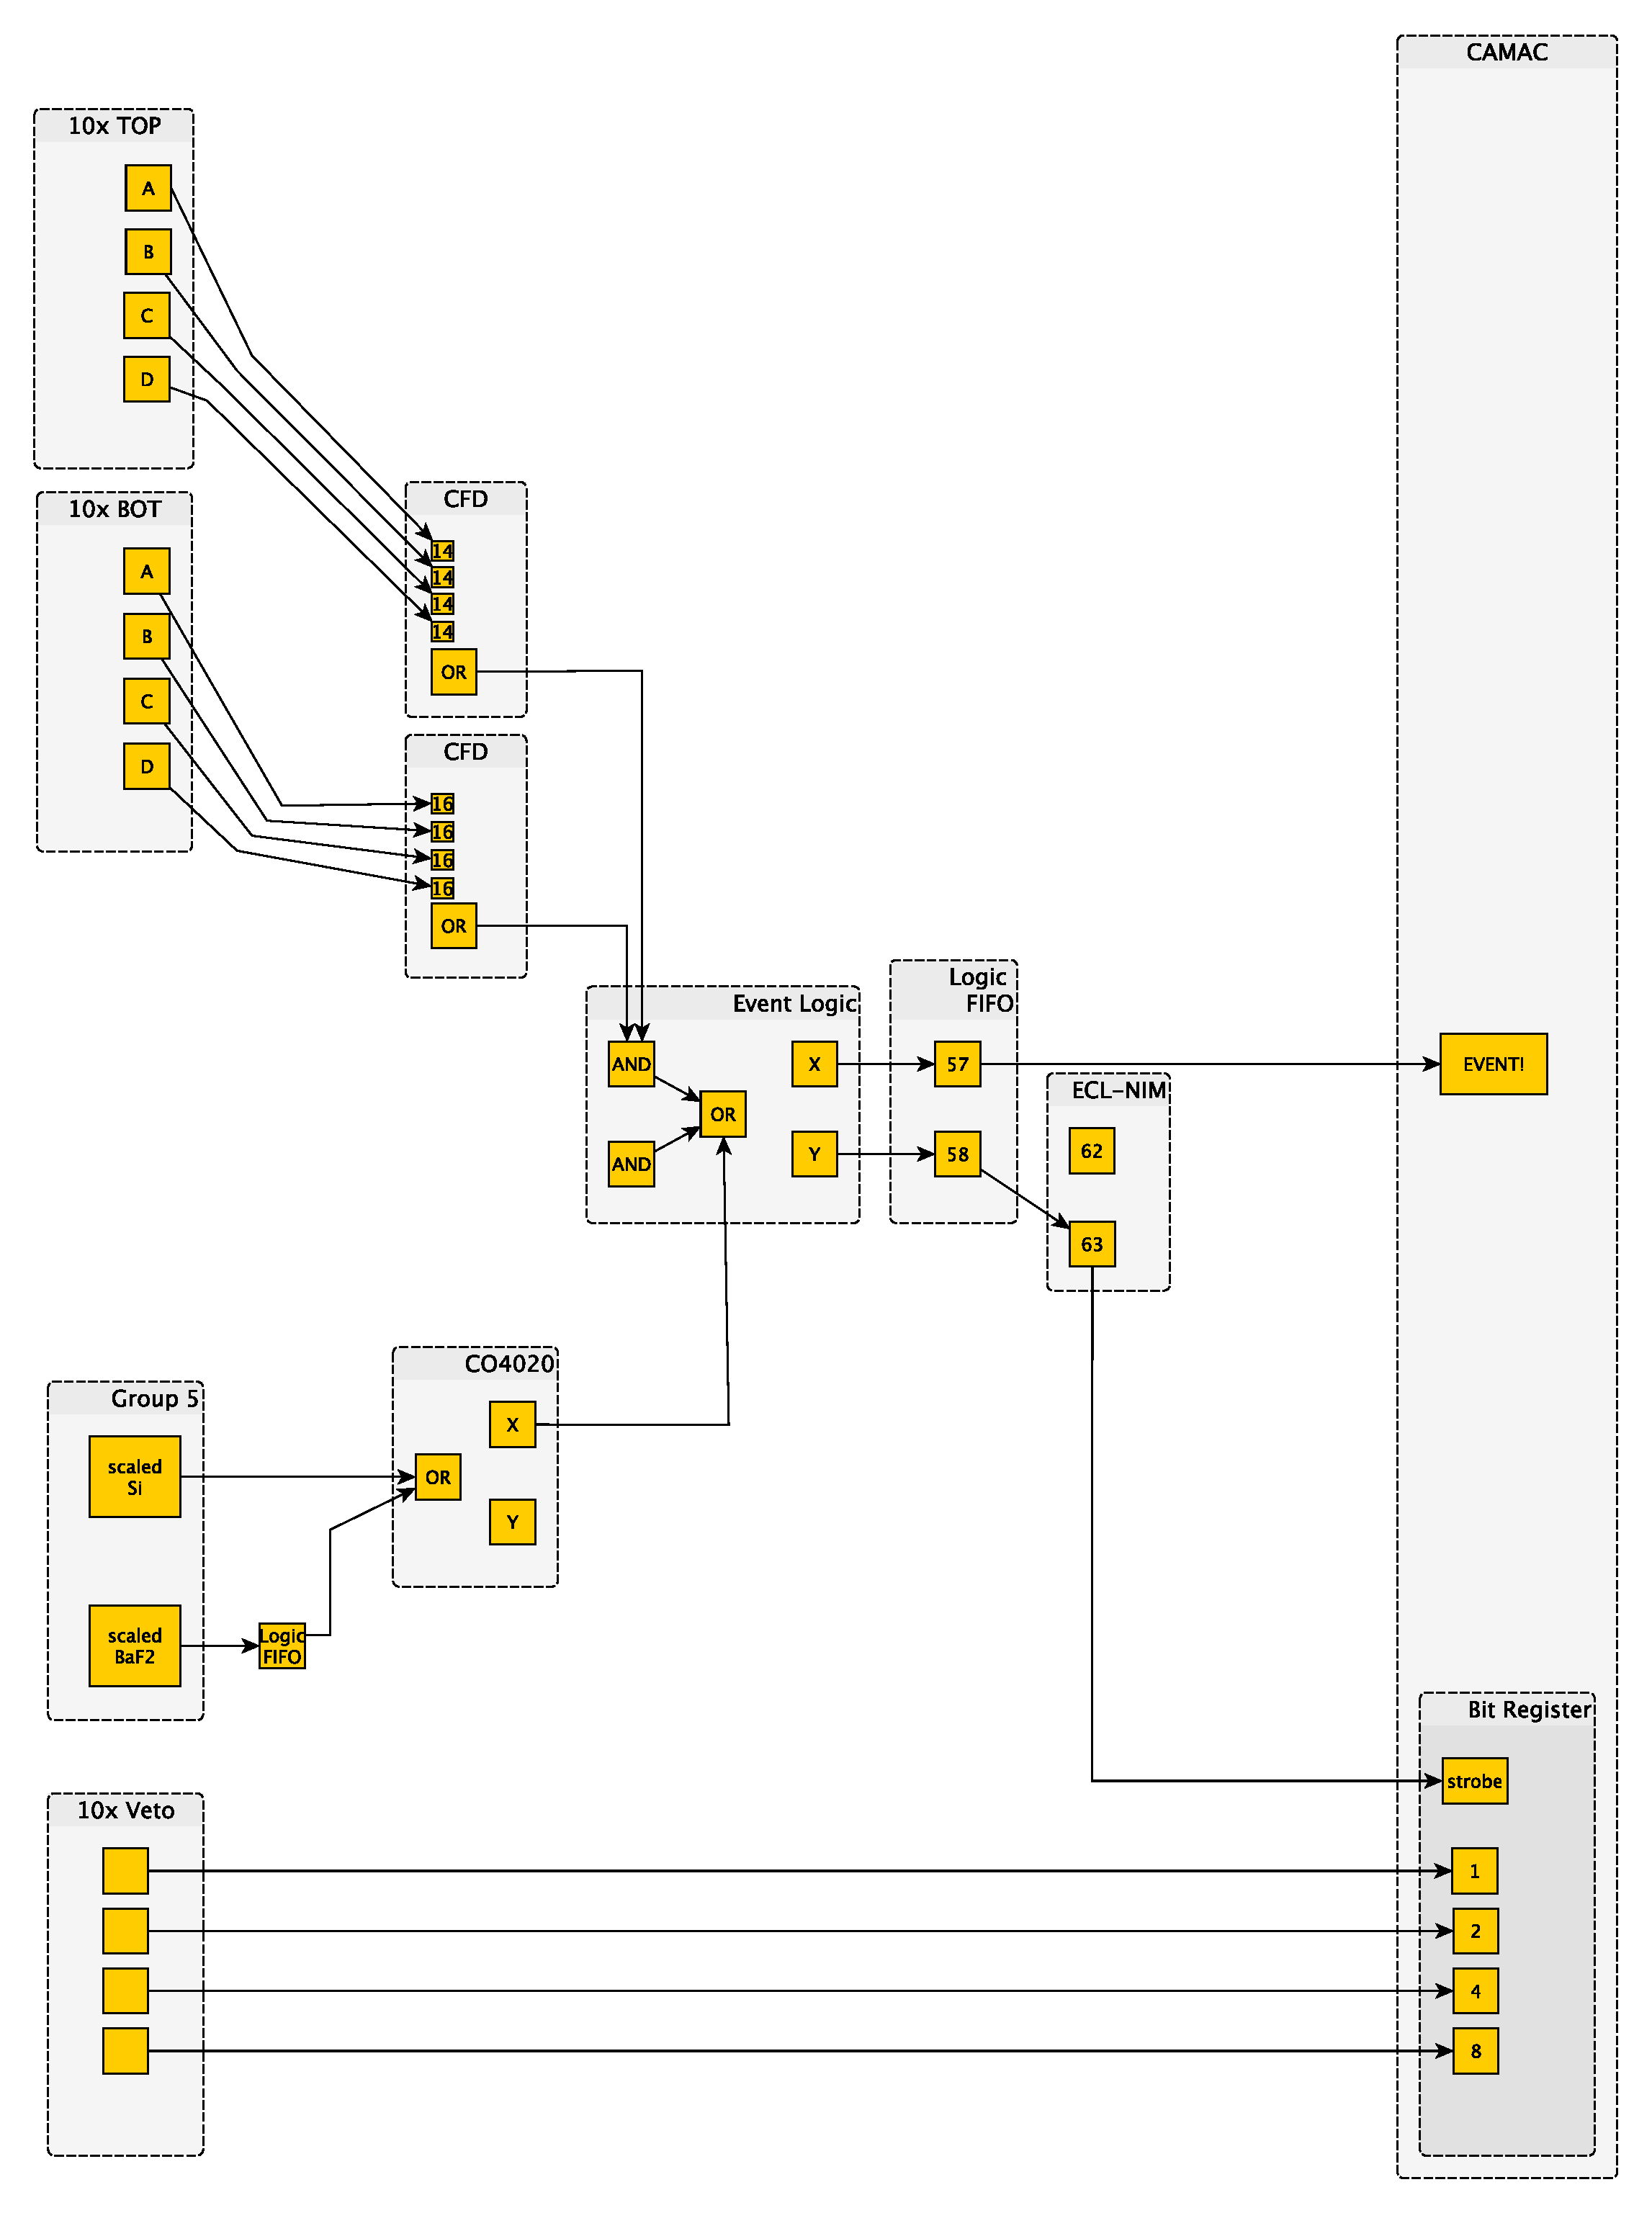
\includegraphics[width=1.0\textwidth]{figures/electronics_veto.eps}
\caption{The integration of the veto electronics with the existing DAQ.  The bit register is used in the data analysis.  Scalers are also added for run-time monitoring.}
\label{fig:vetoElectronics}
\end{figure}
 

\section{Beam Tests}
\begin{comment}
What data should I show?  Old Mg vs. New Mg?  Or New Mg with no veto vs.  New Mg with veto?
show the vetoed spectrum - put a limit on how much real signal is rejected?
\end{comment}
The final veto system reduces the background by approximately a factor of 10 as can be seen in {\fig}~\ref{fig:veto_26Mg}.  The rejection is strongly dependent on energy cuts placed on data, as shown in {\fig}~\ref{fig:vetoRejection_vs_energyCut}.  The veto is less effective at lower energy cuts because $\gamma$ radiation becomes a significant contributor to the random background.  Placing energy cuts above the thorium edge, the Compton edge resulting from the maximally scattered 2.6~MeV $\gamma$ \cite{PDG} from a natural thorium source, rejects much of the room $\gamma$ background.  Although such a high cut on the energy discards on the order of half the neutron events, it maximizes the signal/background ratio.  The reduced background significantly improves the data we were able to obtain on \MgReaction.  Errors on the ground state transition were reduced from 7\% to 3\%.
\begin{figure}[htp]
\centering
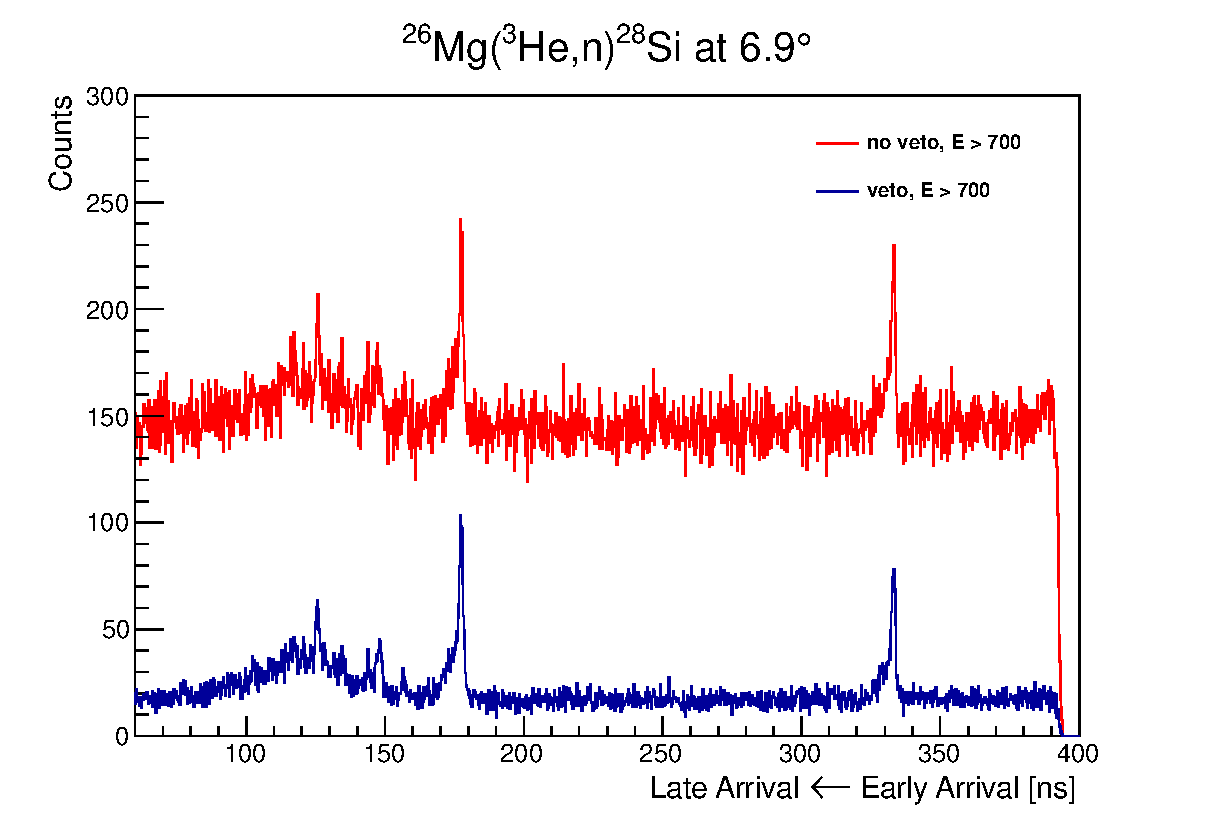
\includegraphics[width=5in]{figures/veto_26Mg.eps}
\caption{\label{fig:vetoData}The effect of the veto on the $^{26}$Mg($^3$He,n) data.}
\label{fig:veto_26Mg}
\end{figure}
  

\subsection{Rejected Signal}
\begin{comment}
Two causes for rejected signal

1. the bars are ganged together; could get a signal in one veto bar that does not mean there was a cosmic in its adjacent neutron detector
2. randoms

can place a limit on randoms, reals, and therefore good rejected signal
\end{comment}
While the achieved background rejection is excellent, it is important to consider how often the veto rejects real neutron events.  Such a rejection could occur when a neutron interacts in both the veto and the neutron detector, when the neutron detector sees a real signal and the veto triggers from an uncorrelated event such as a background $\gamma$-ray, or when a neutron interacting in the detector ejects a proton that triggers the veto.  This last case should occur very rarely; this is the primary reason we chose to mount the veto on the front of the detector.    In these cases, the vetoing of real events will result in timing peaks on top of the flat, random background of the rejected events.  Cases where the veto to wide-angle scatter a neutron that could otherwise interact in the detector will not contribute to a timing peak, but this occurs rarely and is not considered here.  {\fig}~\ref{fig:rejectionTOF} shows the rejected events for all current \Mg{26} data; no peak is visible.  Given the background, this places a limit on the total rejection of real neutron events at ?? at a 90\% confidence level.  
\begin{figure}[htp]
\centering
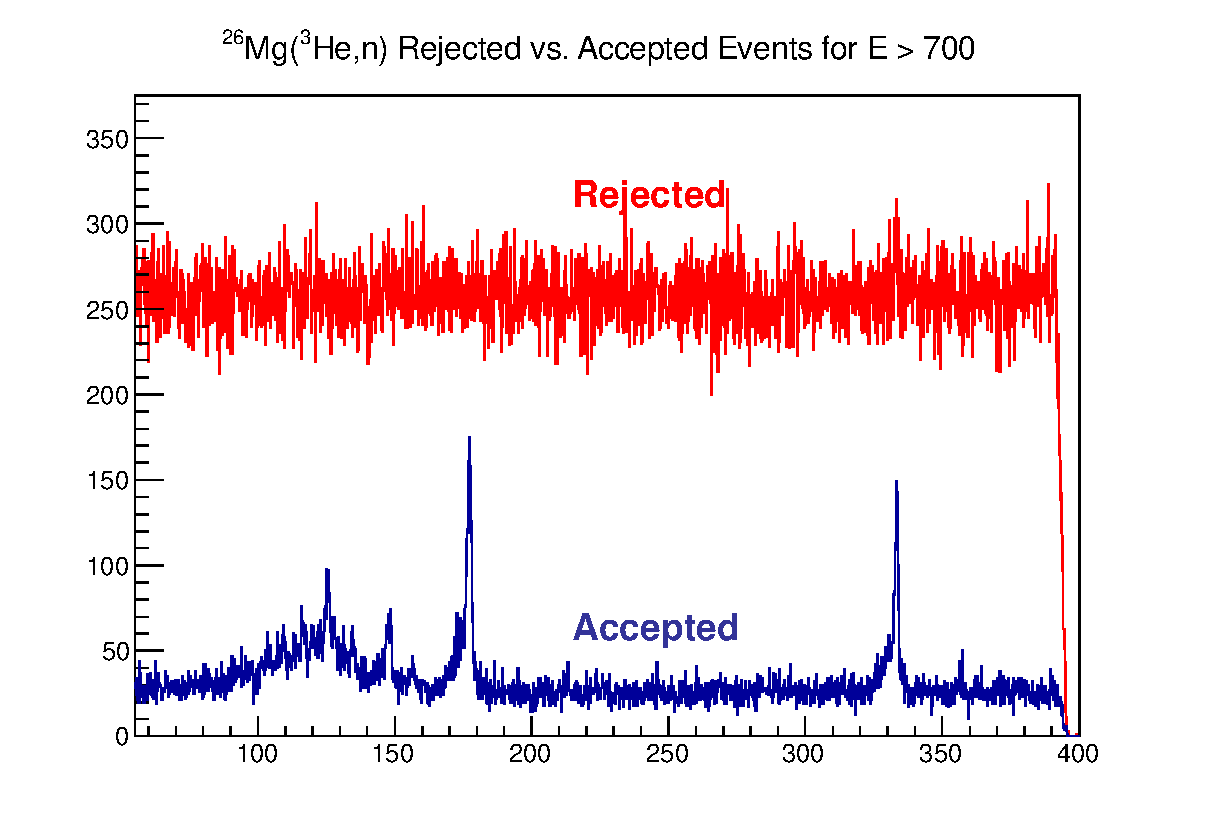
\includegraphics[width=5in]{figures/26Mg_rejection.eps}
\caption{\label{fig:rejection}A plot of the rejected events.  Peaks in the rejected spectrum are from real, vetoed events.  No neutron peak is visible; there is a small peak from rejected gamma events.}
\label{fig:rejectionTOF}
\end{figure}

Testing with \MgReaction demonstrates that the muon veto reduces background by approximately a factor of 10 and does not veto a significant number of beam-related events.  In addition to verifying the proper functioning of the veto system, this reaction also measures the efficiency of the neutron detector because the cross-section is well known.  These efficiency calculations, as well as the data from the \GeTargets experiments, will be discussed in the next chapter.


% % uncomment the following lines,
% if using chapter-wise bibliography
%
% \bibliographystyle{ndnatbib}
% \bibliography{example}
